\subsection{Implementation of a point-to-point communication between a moving train and a station}

\begin{frame}{Preliminary Work}{Implementation of a point-to-point communication between a moving train and a station}
\begin{block}{\textbf{Implementation of a point-to-point communication between a moving train and a station}}
	
	\begin{figure}[ht!]
		\centering
			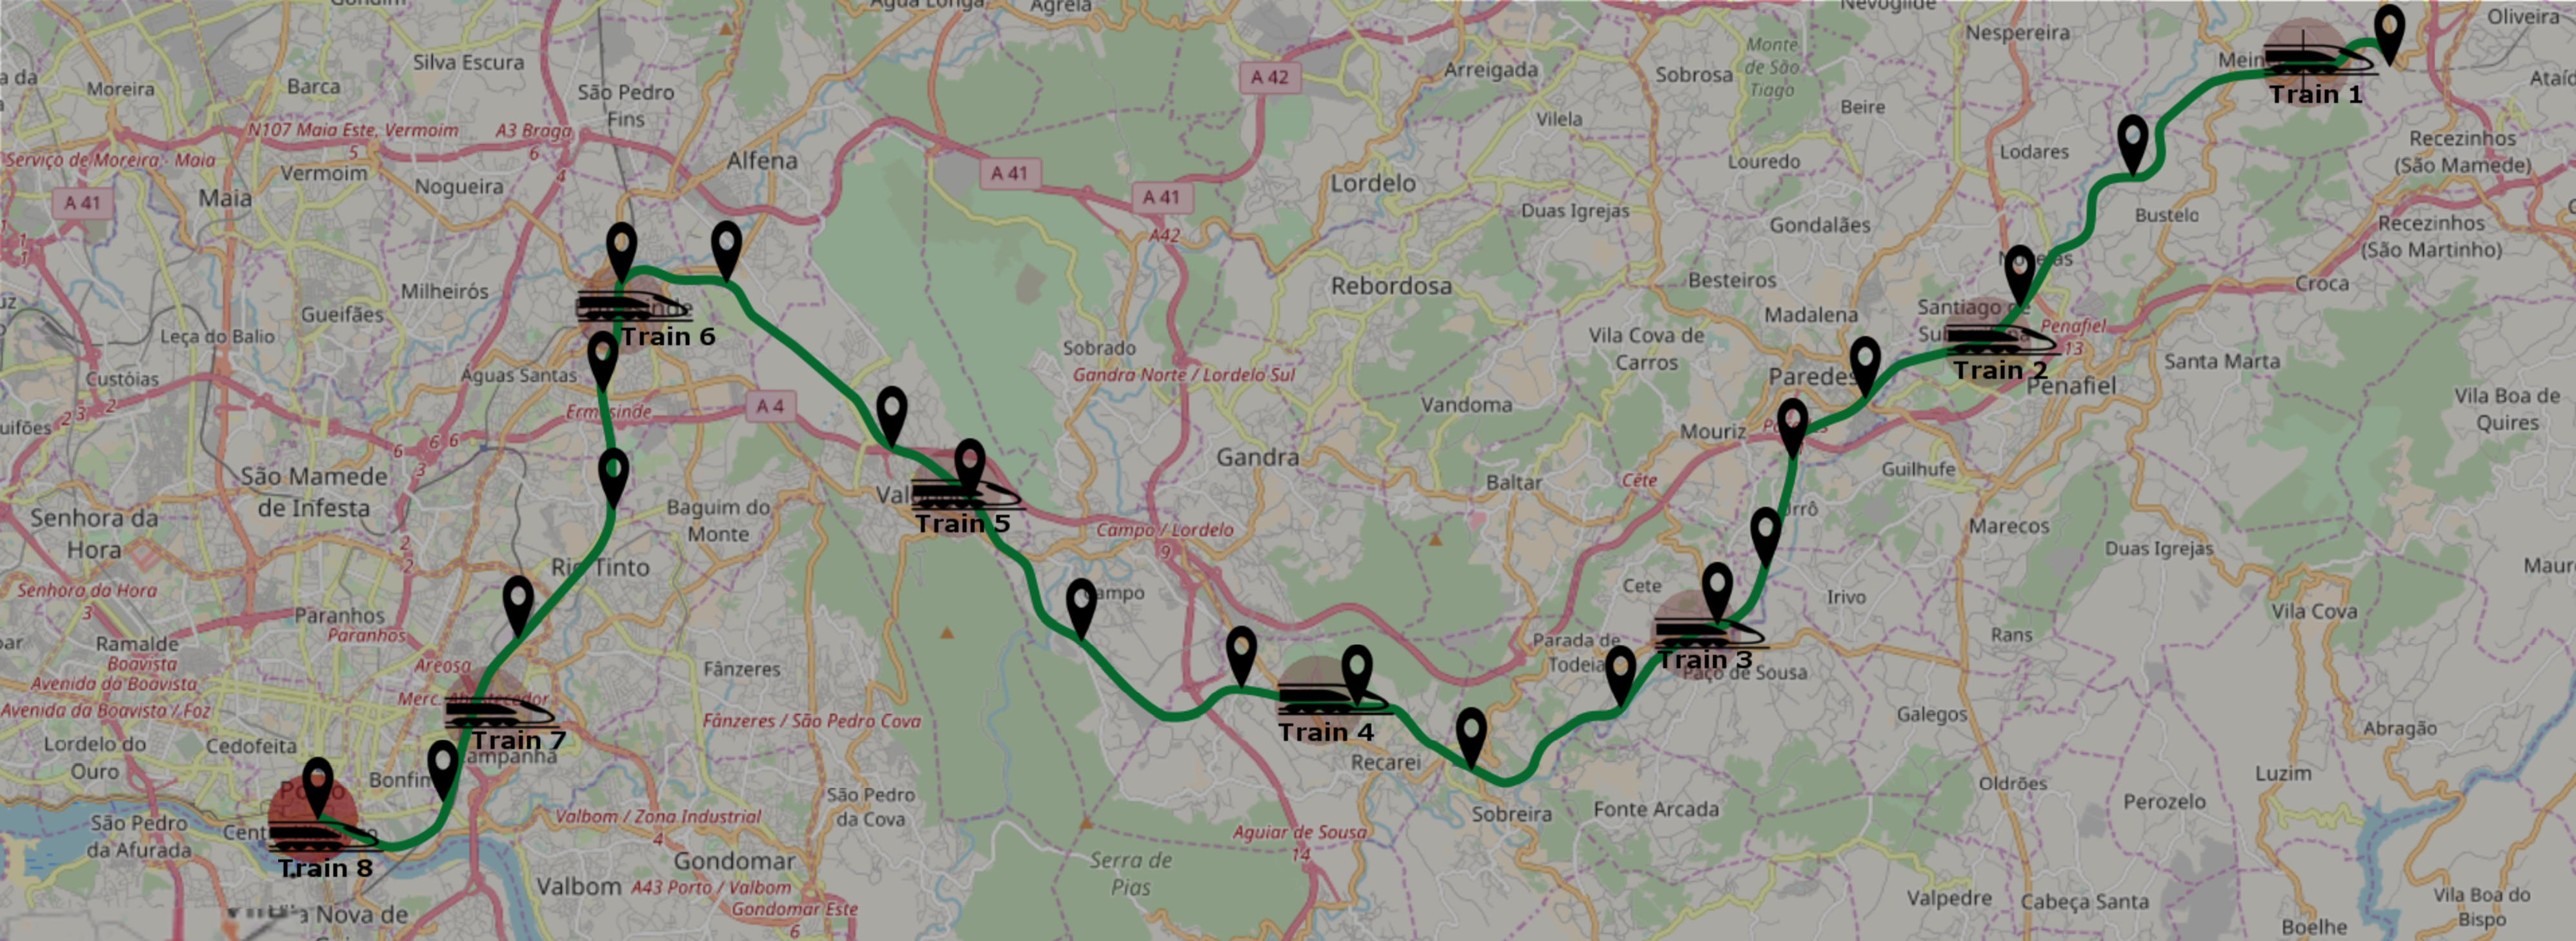
\includegraphics[width=0.9\textwidth,keepaspectratio]{figures/50.PreliminaryW/porto-caide2}
		\caption{Porto-Caíde railway line: simulation using OMNeT++ network simulator.}
	\end{figure}
	
\end{block}
\end{frame}
%%%%%%%%%%%%%%%%%%%%%%%%%%%%%%%%%%%%%%%%%%%%%%%%%%%%%%%%%%%%%%%%%%%%%%%%%%%%%%%%%%%%%

\begin{frame}{Preliminary Work}{Implementation of a point-to-point communication between a moving train and a station}

\begin{figure}[ht!]
	\centering
	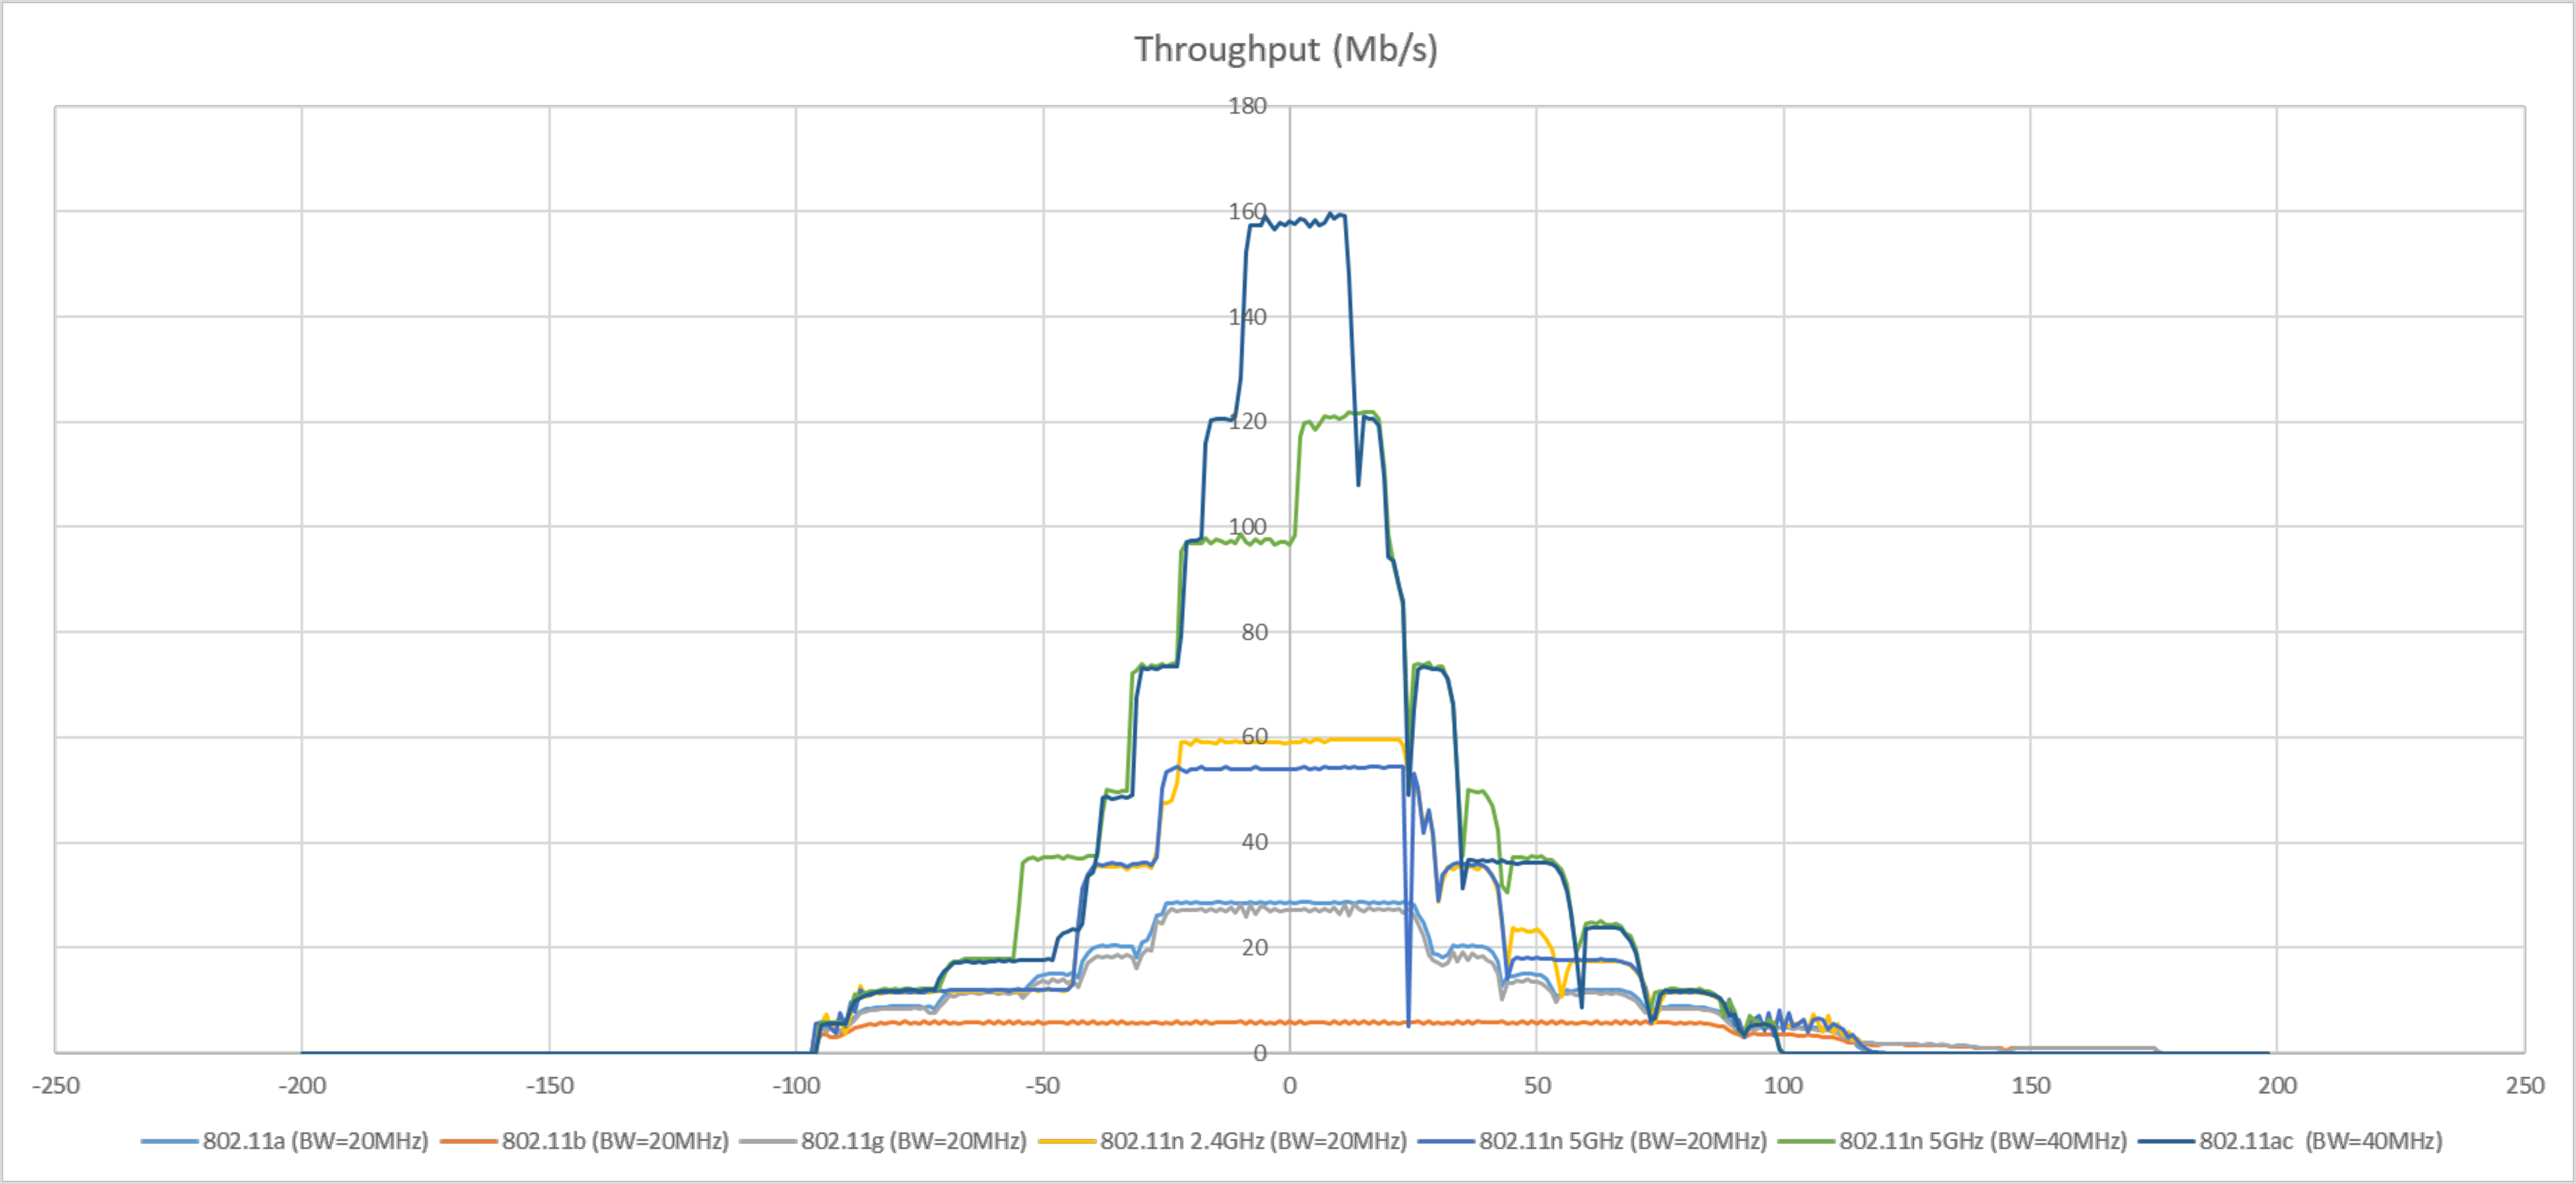
\includegraphics[width=\textwidth,keepaspectratio]{figures/50.PreliminaryW/distance-rate}
	\caption{Evaluation of moving node for different 802.11 network standards using NS-3.}
\end{figure}


\end{frame}
%%%%%%%%%%%%%%%%%%%%%%%%%%%%%%%%%%%%%%%%%%%%%%%%%%%%%%%%%%%%%%%%%%%%%%%%%%%%%%%%%%%%%

\begin{frame}{Preliminary Work}{Implementation of a point-to-point communication between a moving train and a station}

\begin{figure}[ht!]
	\centering
	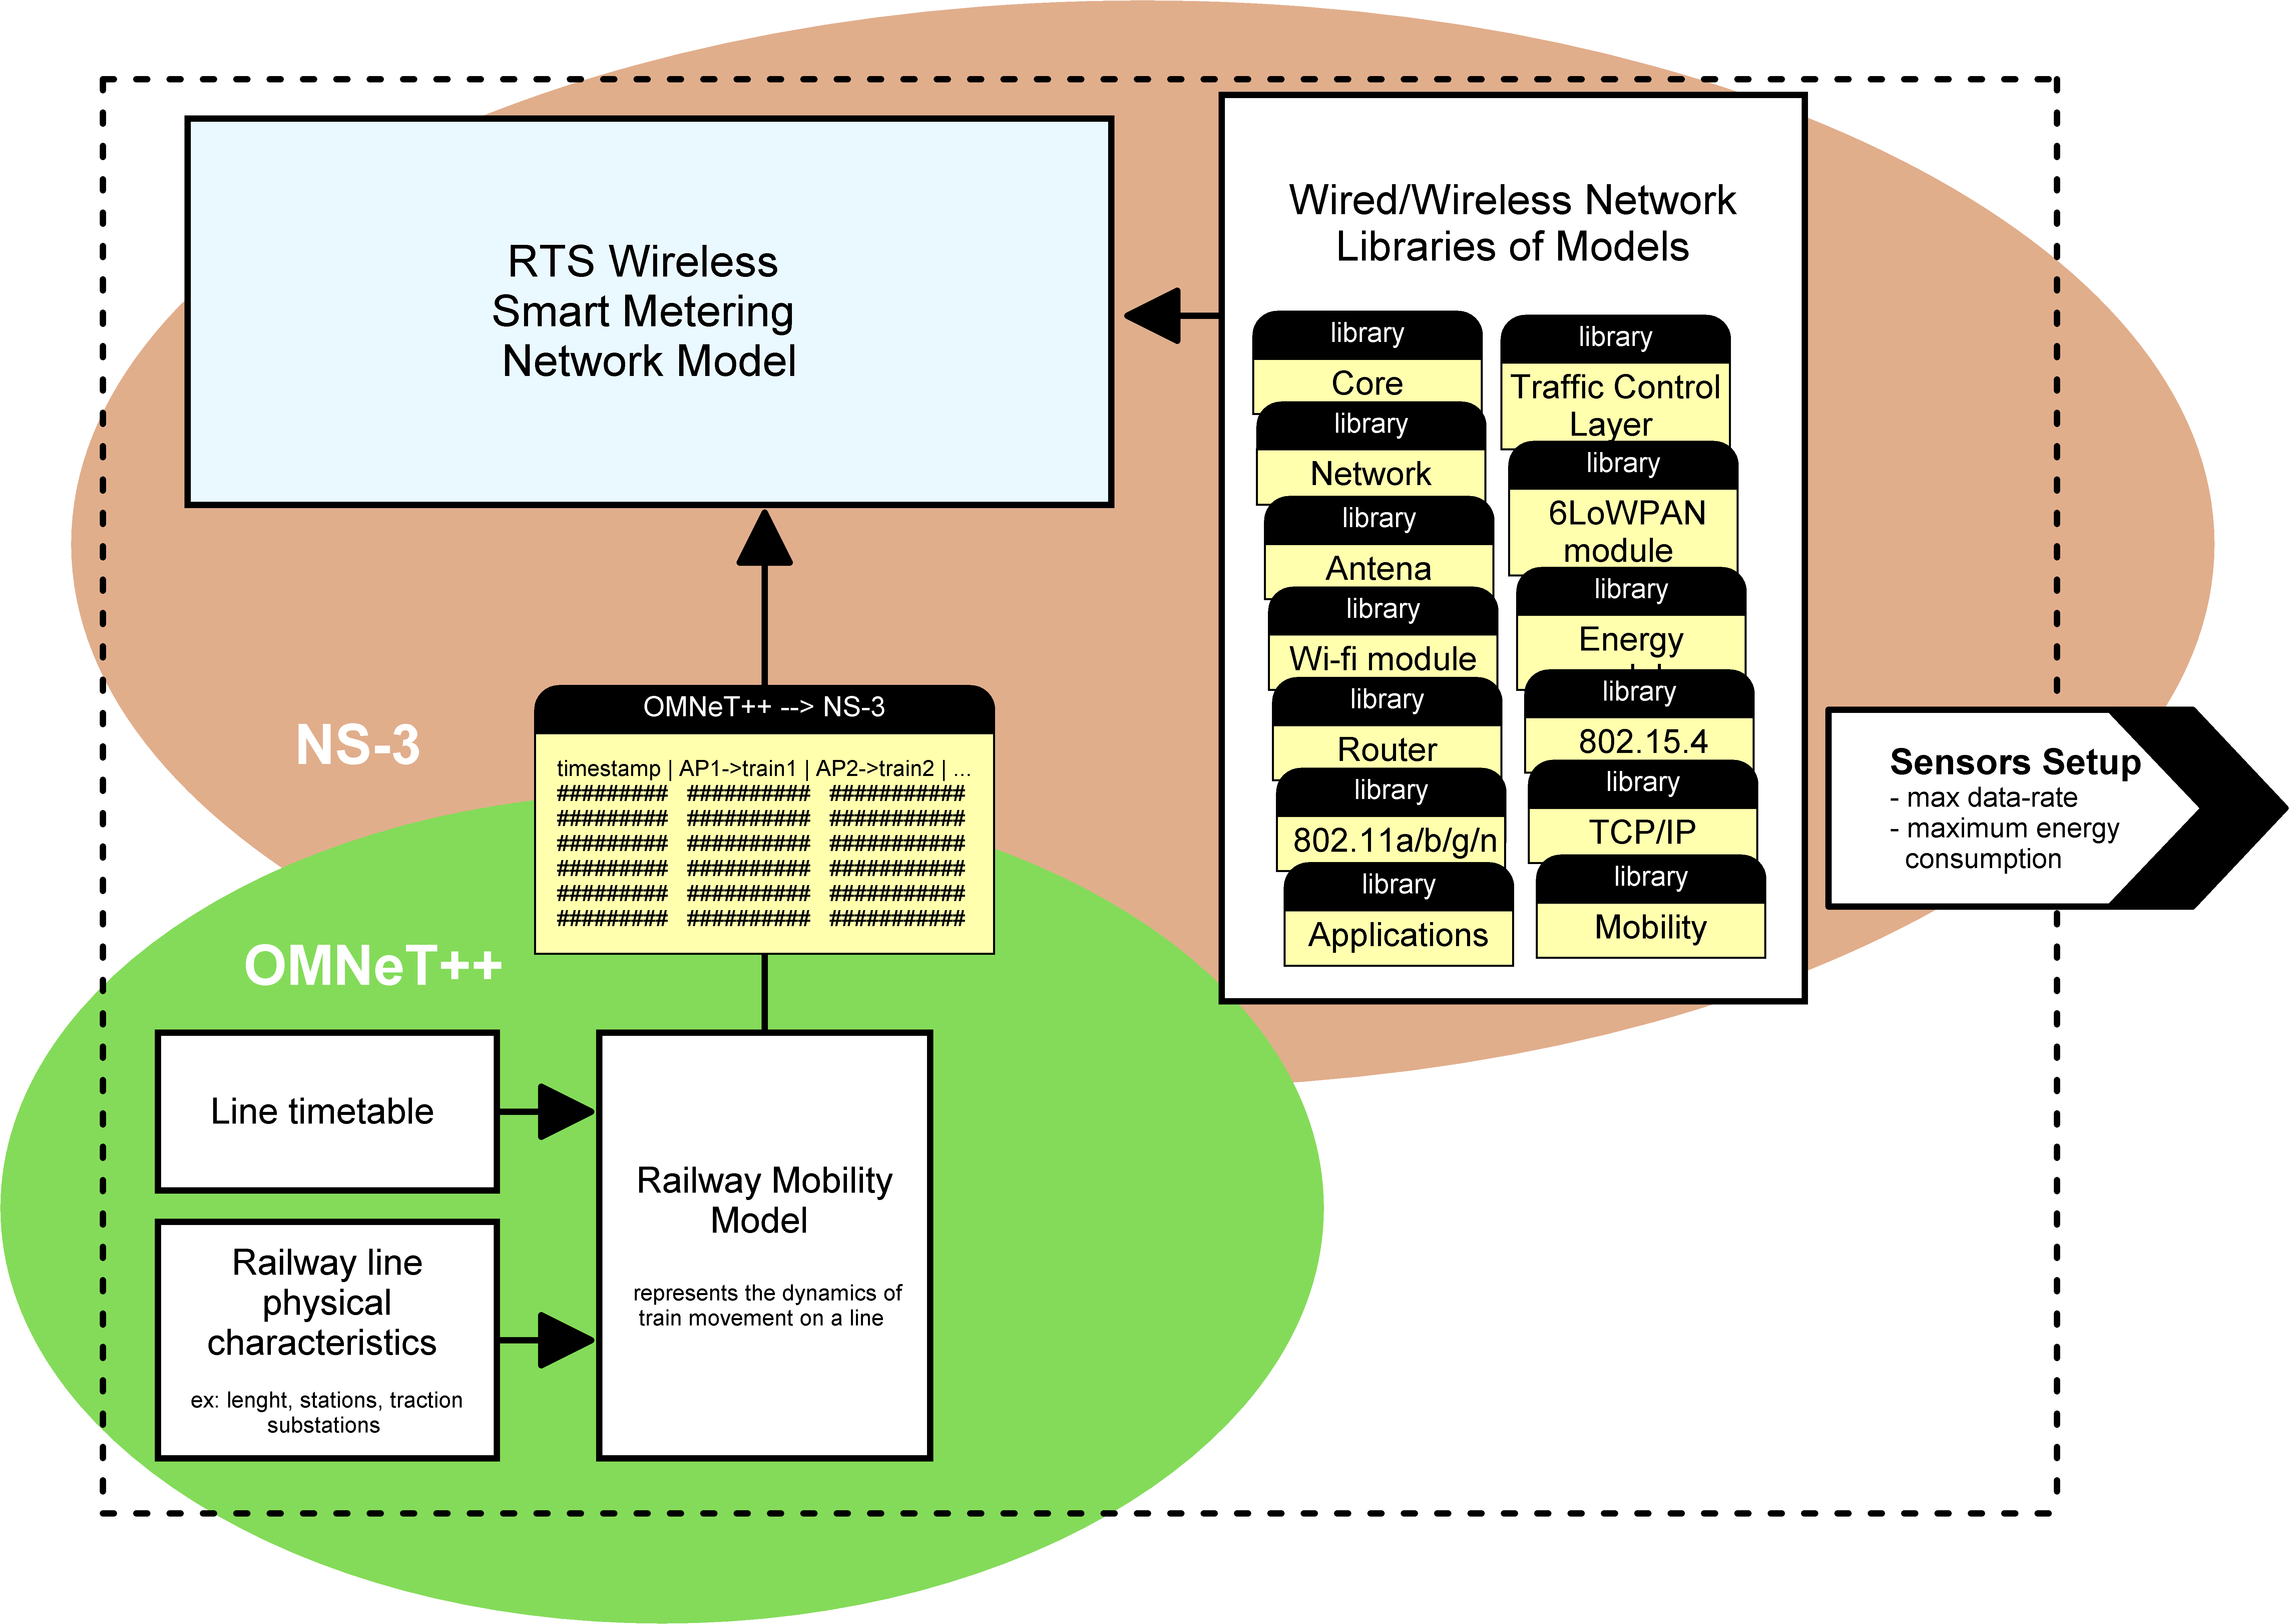
\includegraphics[width=0.70\textwidth,keepaspectratio]{figures/50.PreliminaryW/omnetpp+ns32}
	\caption{Simulator layers: proposed solution using OMNeT++ and NS-3.}
\end{figure}


\end{frame}
%%%%%%%%%%%%%%%%%%%%%%%%%%%%%%%%%%%%%%%%%%%%%%%%%%%%%%%%%%%%%%%%%%%%%%%%%%%%%%%%%%%%%

\subsection{Evaluation of the non-intrusive voltage sensor}

\begin{frame}{Preliminary Work}{Evaluation of the non-intrusive voltage sensor}
\begin{block}{\textbf{Evaluation of the non-intrusive voltage sensor}}
	
		\begin{minipage}[t]{0.35\linewidth}
		
		\begin{figure}[ht!]
			\centering
				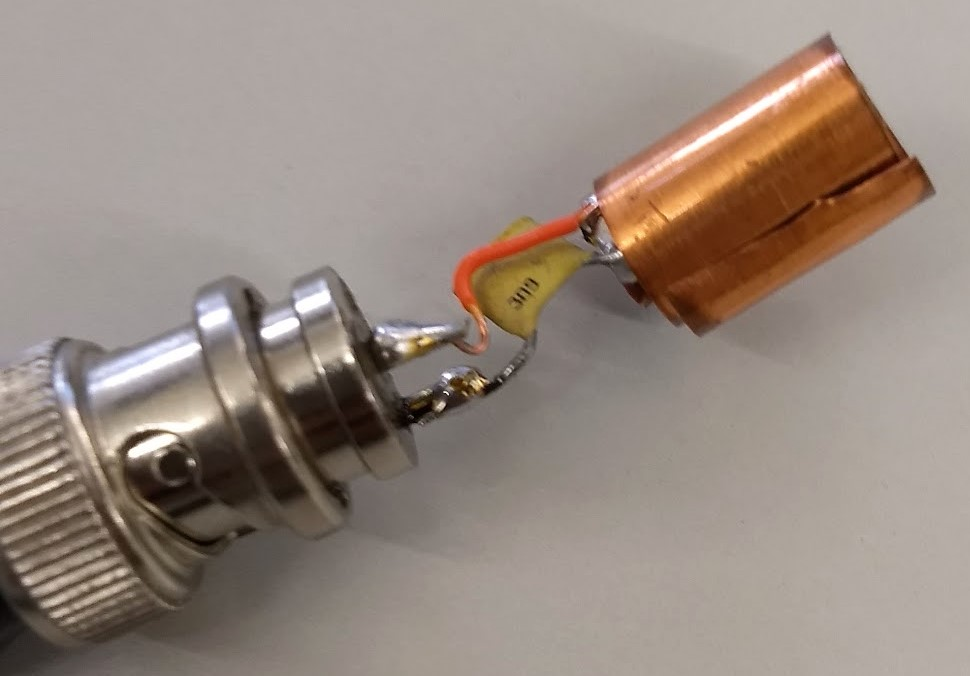
\includegraphics[width=0.6\textwidth,keepaspectratio]{figures/50.PreliminaryW/voltage_sensor}
			%		\vspace{2em}
			\caption{Photo of implemented non-intrusive voltage sensor.}
		\end{figure}
	\end{minipage}\hfill
	\begin{minipage}[t]{0.50\linewidth}
		%\begin{itemize}
		%	\item  50 Hz 25 kV supply system.
		
		%\end{itemize}
		
		\begin{figure}[ht!]
			\centering
			\includegraphics[width=0.9\textwidth,keepaspectratio]{figures/50.PreliminaryW/generalArchitecture}
			\caption{Signal conditioning and digital processing architecture.}
		\end{figure}
		
		
		
	\end{minipage}
	
	
	
\end{block}
\end{frame}
%%%%%%%%%%%%%%%%%%%%%%%%%%%%%%%%%%%%%%%%%%%%%%%%%%%%%%%%%%%%%%%%%%%%%%%%%%%%%%%%%%%%%

\begin{frame}{Preliminary Work}{Evaluation of the non-intrusive voltage sensor}
\begin{figure}[h!]
	\centering
	\begin{minipage}{.48\textwidth}
		\centering
		%		\vspace{2.5em}
		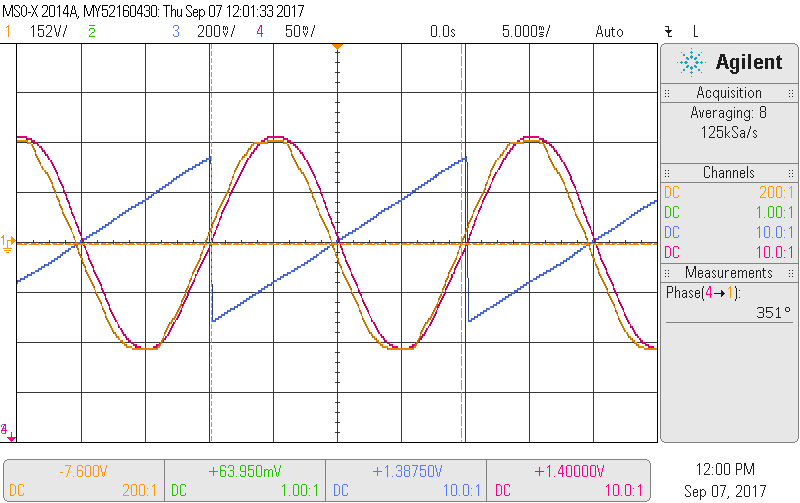
\includegraphics[width=0.95\textwidth,keepaspectratio]{figures/50.PreliminaryW/scope_9}
		%		\vspace{2em}
		\captionof{figure}{Waveforms of AC voltage (orange), estimated voltage (pink) and estimated phase angle (blue) without phase compensation.}
		\label{fig:5.scope_9}
	\end{minipage}%
	\begin{minipage}{.01\textwidth}  ~\end{minipage}	
	\begin{minipage}{.48\textwidth}
		\centering
		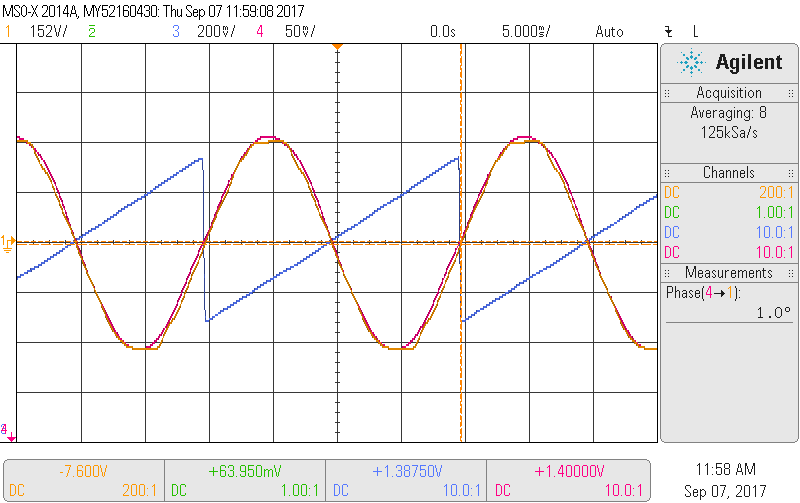
\includegraphics[width=0.95\textwidth,keepaspectratio]{figures/50.PreliminaryW/scope_10}
		%		\vspace{2em}
		\captionof{figure}{Waveforms of AC voltage (orange), estimated voltage (pink) and estimated phase angle (blue) with phase compensation.}
		\label{fig:5.scope_10}
	\end{minipage}
\end{figure}
\end{frame}
%%%%%%%%%%%%%%%%%%%%%%%%%%%%%%%%%%%%%%%%%%%%%%%%%%%%%%%%%%%%%%%%%%%%%%%%%%%%%%%%%%%%%
